\documentclass[conference]{IEEEtran}
\IEEEoverridecommandlockouts
% The preceding line is only needed to identify funding in the first footnote. If that is unneeded, please comment it out.
%Template version as of 6/27/2024

\usepackage{cite}
\usepackage{amsmath,amssymb,amsfonts}
\usepackage{pxfonts}
\usepackage{algorithmic}
\usepackage{graphicx}
\usepackage{textcomp}
\usepackage{xcolor}
\usepackage[main=brazil,english]{babel}
\def\BibTeX{{\rm B\kern-.05em{\sc i\kern-.025em b}\kern-.08em
    T\kern-.1667em\lower.7ex\hbox{E}\kern-.125emX}}
\begin{document}

\title{
	%Aplicação de CNNs no reconhecimento de gestos a partir de sinais de sEMG
	%Revisão da aplicação de CNN no reconhecimento de sinais de sEMG
	%Reconhecimento de gestos a partir de sinais sEMG: uma revisão de aplicações de CNN
	%Uso de CNNs para reconhecimento de gestos a partir de sinais sEMG
	%Uso de CNNs para reconhecimento de gestos a partir de sinais sEMG: revisão
	%Revisão da arquitetura CNN para aplicações de sEMG: resultados e observações
	%2.
	%Reconhecimento de gestos por sEMG: uma análise da eficiência de arquiteturas de CNNs
	%Avanço no reconhecimento de gestos por sEMG: uma revisão de desempenho de CNNs
	%1.
	%Eficiência de CNNs no reconhecimento de gestos por sEMG: uma revisão de estudos recentes
	%3.
	%CNNs aplicadas ao reconhecimento de gestos por sEMG: Avaliação de desempenho e eficiência
	%4.
	%Reconhecimento de gestos por sEMG: uma análise da eficiência de CNNs em estudos recentes
	%5
	%Reconhecimento de gestos por sEMG com CNNs: uma análise de eficiência em estudos recentes
	%6
	%Reconhecimento de Gestos por sEMG: Uma Análise da Eficiência de CNNs 
	%7
	Processamento de Imagens para Detecção de Furos em Bicos Injetores Diesel
	%Panorama da eficiência em reconhecimento de gestos por sEMG: uma revisão de abordagens com CNNs
	 
%{\footnotesize \textsuperscript{*}Note: Sub-titles are not captured for https://ieeexplore.ieee.org  and
%should not be used}
%\thanks{Identify applicable funding agency here. If none, delete this.}
}

\author{
	\IEEEauthorblockN{
		1\textsuperscript{st}
		Wellinthon da Silveira Kiiller
	}
	\IEEEauthorblockA{
		\textit{Programa de Pós-Graduação em Engenharia Elétrica e
		Informática Industrial (CPGEI-CT)} \\
		\textit{Universidade Tecnológica Federal do Paraná (UTFPR)}\\
		Curitiba, Paraná, Brasil \\
		https://orcid.org/0009-0000-8591-0393
	}
	%\and
	%\IEEEauthorblockN{2\textsuperscript{nd} Given Name Surname}
	%\IEEEauthorblockA{\textit{dept. name of organization (of Aff.)} \\
	%\textit{name of organization (of Aff.)}\\
	%City, Country \\
	%email address or ORCID}
}

\maketitle

% Linguagem: português
%\selectlanguage{brazil}
%\renewcommand\IEEEkeywordsname{Palavras-chave}
%\begin{abstract}
	%Contexto e motivação
	%O que é o tema e por que ele é importante?
	%O reconhecimento de gestos a partir de sinais de eletromiografia de superfície (sEMG) tem ganhado destaque em aplicações biomédicas, especialmente no controle de próteses e em sistemas de reabilitação.	
	%Objetivo do trabalho
	%O que você fez? Qual era o propósito principal?
	%Esse trabalho investiga a aplicação de redes neurais convolucionais (CNNs) na identificação e classificação de gestos com base em sinais de sEMG.	
	%Metodologia usada
	%Como você fez? Qual foi a abordagem geral?
	%Por meio de uma revisão de literatura, são analisadas arquiteturas de CNN comumente empregadas na área, como ResNet-50, VGGNet-11 e GoogLeNet, considerando diferentes métodos de pré-processamento e representação dos sinais em imagens. Além disso, são discutidas técnicas como \textit{sliding window} e transformadas tempo-frequência, incluindo a \textit{Short-Time Fourier Transform} (STFT).
	%Principais resultados (se houver)
	%Quais foram os achados mais relevantes?
	%(Se não houver resultados ainda, diga o que o artigo apresenta.)
	%Os resultados apresentados em pesquisas recentes fortalecem o alto potencial das CNNs em alcançar acurácias superiores a 90\% no reconhecimento de padrões gestuais, com perspectivas promissoras para aplicações em tempo real.
	%Conclusão ou contribuição
	%O que esse trabalho oferece à área? Qual é a contribuição?
	%Por fim, esse trabalho oferece uma base metodológica sólida, servindo como referência para futuras implementações de sistemas de reconhecimento de movimentos baseados em sEMG.
%\end{abstract}

%\begin{IEEEkeywords}
%CNN, sEMG, classificação de gestos, reconhecimento de padrões.
%\end{IEEEkeywords}

% Linguagem: português
\selectlanguage{brazil}

\section{Introducão}

Os bicos injetores desempenham uma função fundamental nos sistemas de combustão a diesel. Em uma multinacional especializada na produção desses bicos, é essencial assegurar a rastreabilidade do produto ao longo dos diversos processos de fabricação. Uma forma eficaz de garantir a rastreabilidade é por meio de gravações a laser, que, ao contrário de etiquetas ou adesivos, permanece intacta durante o processo de fabricação.

Nesse contexto, este trabalho tem como objetivo demonstrar a aplicação de técnicas de processamento de imagens para detectar furos na superfície de vedação de bicos injetores diesel, uma área estratégica para a gravação a laser com fins de rastreabilidade. O artigo está organizado da seguinte forma: na Seção 2.A, é apresentada uma breve explicação sobre os bicos injetores; an Seção 2.B, são descritas as técnicas de processamento de imagens utilizadas; por fim, a Seção de Considerações Finais encerra o artigo, destacando as contribuições do estudo.

\cite{karhub}

\section{Metodologia}
\subsection{Bico Injetor Diesel}

A Figura \ref{fig:bico-injetor-real} ilustra um modelo de bico injetor, um dos principais componentes de um sistema de combustão a diesel. Como o foco deste trabalho é a aplicação de técnicas de processamento de imagens, o funcionamento do injetor não será abordado em detalhes. No entanto, a Figura \ref{fig:bico-injetor} destaca alguns de seus componentes.

A Figura \ref{fig:bico-injetor} destaca as seguintes regiões do bico injetor: base (1), haste (2), cúpula (3), furos de fixação (4 e 5), furo de injeção de combustível (6), guia do corpo (7), furo cego (8), assento da agulha (9), ponta da agulha (10), guia da agulha (11) e espiga da agulha (12) \cite{Girotto2023}. Os furos de fixação (4 e 5) e injeção de combustível (6) estão localizados em uma região chamada de superfície de vedação, conforme ilustra a Figura \ref{fig:superficie-de-vedacao}.

\begin{figure}[t]
 	\centering
 	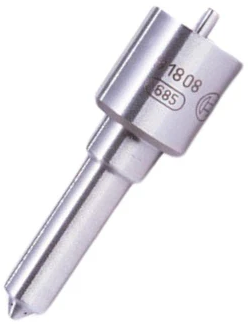
\includegraphics[scale=0.5]{Images/bico-injetor-real.png}
 	\caption{Bico injetor diesel. Fonte: \cite{karhub}.}
 	\label{fig:bico-injetor-real}
\end{figure}
 
\begin{figure}[t]
	\centering
	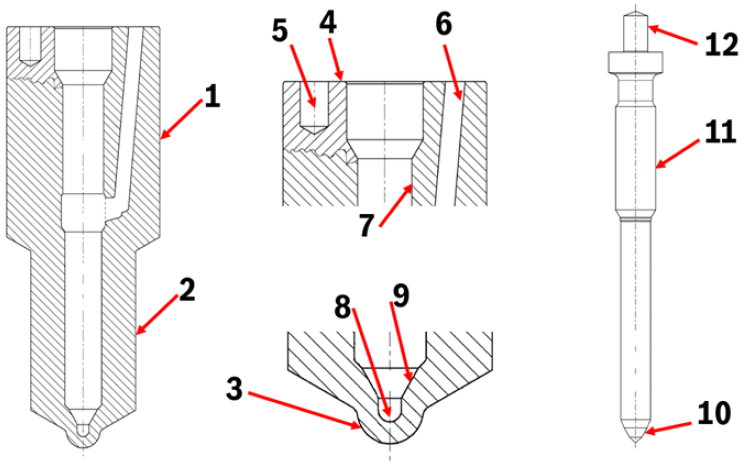
\includegraphics[scale=0.4]{Images/bico-injetor.png}
	\caption{Componentes de um bico injetor diesel. Fonte: \cite{Girotto2023}.}
	\label{fig:bico-injetor}
\end{figure}

\begin{figure}[t]
	\centering
	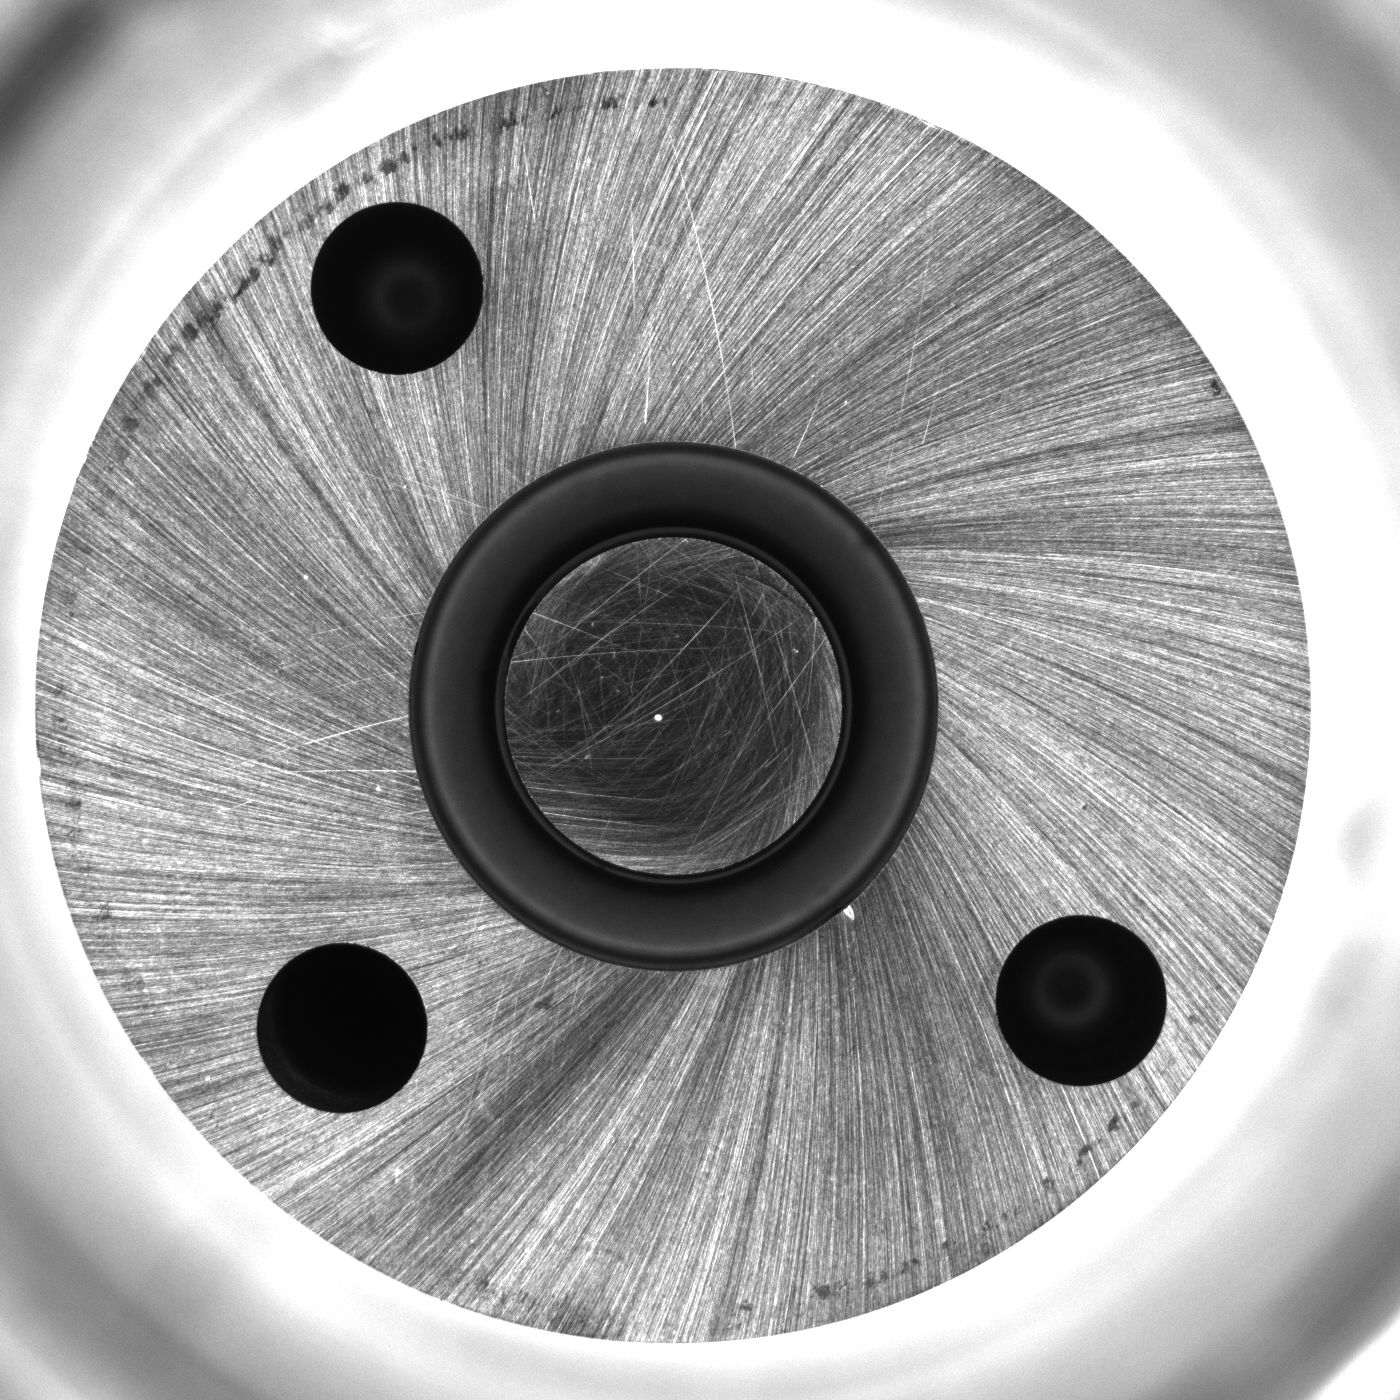
\includegraphics[scale=0.10]{Images/superficie-de-vedacao.jpg}
	\caption{Bico injetor diesel}
	\label{fig:superficie-de-vedacao}
\end{figure}

\section*{Considerações Finais}
%Esse trabalho teve como objetivo analisar a eficiência das CNNs no reconhecimento de gestos com base em sinais de sEMG. Os fundamentos apresentados, bem como as metodologias de pré-processamento e conversão dos sinais em imagens - como o uso de janelas deslizantes e transformadas tempo-frequência - demonstraram impacto direto na performance dos modelos. Essas técnicas, aliadas aos benefícios das redes convolucionais, permitiram alcançar ótimos resultados, com acurácias superiores a 0,8 em pesquisas recentes.

%%%%%%%%%%%%%%%%%%%%%%%%%%%%%%%%%%%%%%%%%%%%%%%%%%%%%%%%%%%%%%%%%%%%%%%%%%%%%%%%%%%%%%%%%%%%%%
%\section*{References}
\bibliographystyle{IEEEtran}
\bibliography{references}

%\begin{thebibliography}{00}
%\end{thebibliography}

%\vspace{125pt}
%\color{red}
%IEEE conference templates contain guidance text for composing and formatting conference papers. Please ensure that all template text is removed from your conference paper prior to submission to the conference. Failure to remove the template text from your paper may result in your paper not being published.

\end{document}
